\section{Physical Implementation (ab)}
\label{sec:PCB-implementation}

The final, delivered module is a $88mm\times62mm$ PCB. The PCB manufactured 
for the project was done so for free, using Spirit Circuits' "Go Naked"
service \cite{go-naked}. The PCB itself is a "tracks and holes" only service 
- no soldermask or silkscreen is applied. The schematic of the circuit 
delivered is available in Appendix \ref{Payload_Schematic}, and of the PCB layout in Appendix 
\ref{appendix-layout}. A waterproof lacquer will be applied to the PCB to prevent condensation 
from shorting tracks together, and the module itself presented in a 
waterproof container before flight testing.

A quote of \pounds 56.39 has been obtained from PCB Train \footnote{\url{http://www.pcbtrain.co.uk/quote-and-order-pcb/}} 
for a single PCB, with electrical testing, on a 15 day lead time. 
Please note that Spirit Circuits have only manufactured our prototype 
free of charge on a one-off basis. Being impressed with this service, 
we may recommend that clients contact them for a competitive quote.

\begin{figure}[H]
        \centering
        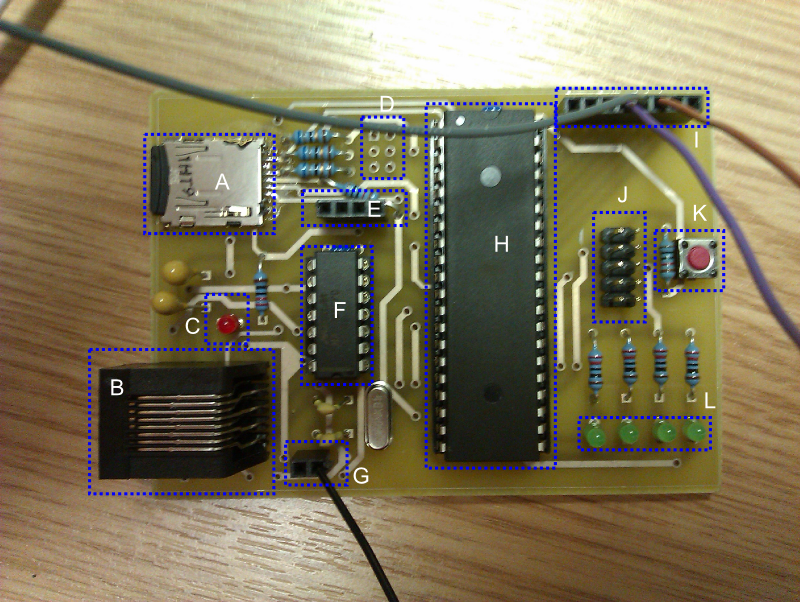
\includegraphics[width=1.00\textwidth]{figures/PayloadImplementation.png}
        \captionof{figure}{Image of the final payload, under test, before lacquer is applied. R11 can be seen between the Camera header and a via near the SD card Vcc.}. 
        \label{fig:PayloadImplementation}
\end{figure}

In figure \ref{fig:PayloadImplementation}, the letters refer to the following 
features of the payload module:

\begin{itemize}
\item \textbf{A:} microSD Card slot
\item \textbf{B:} RJ45 socket, more popularly known as an ethernet socket. 
(Actually implements the RS485 protocol)
\item \textbf{C:} Power LED. Shows whether 3V3 from the ethernet socket is connected.
\item \textbf{D:} ISP programming header socket. As seen, this is not 
soldered on, as we have been using the JTAG header for testing, but will be soldered 
before delivery to the customer.
\item \textbf{E:} Camera header. The camera can be connected to our PCB 
simply by attaching the hook-up wire in the correct order. (L-R: 3V3, GND, 
Camera TX, Camera RX)
\item \textbf{F:} MAX489 (RS485 Transceiver) \footnote{\url{http://uk.farnell.com/9725148}}. 
Cheaper version of the MAX3070 used in the sample peripheral.
\item \textbf{G:} Power header. L: 3V3, R: GND.
\item \textbf{H:} ATmega644P \cite{atmega644p}
\item \textbf{I:} ATmega644P Port A expansion header. (In the image, this is 
being used as a connection to an Arduino Uno so that we may view the debug 
information)
\item \textbf{J:} JTAG programming header
\item \textbf{K:} Reset button
\item \textbf{L:} Debug LEDs
\end{itemize}
